\documentclass[11pt,a4paper]{article}

\usepackage[utf8]{inputenc}
\usepackage[spanish,es-tabla]{babel}
\usepackage[margin=2.0cm]{geometry}
\usepackage{amsmath,amssymb}
\usepackage{graphicx}
\usepackage{booktabs}
\usepackage{tabularx}
\usepackage{hyperref}
\usepackage{xcolor}
\usepackage{float}
\usepackage{caption}
\usepackage{subcaption}
\usepackage{listings}
\usepackage{microtype}
\usepackage{tcolorbox}

\hypersetup{
    colorlinks=true,
    linkcolor=blue!70!black,
    citecolor=blue!70!black,
    urlcolor=blue!70!black
}

\lstset{
    basicstyle=\ttfamily\footnotesize,
    backgroundcolor=\color{gray!10},
    frame=single,
    rulecolor=\color{gray!30},
    breaklines=true,
    showstringspaces=false
}

\title{\textbf{Laboratorio de Análisis de Datos en Redes: \\ Predicción de Congestión en un Enlace LAN Mediante Captura de Tráfico y Regresión Lineal}}
\author{\textbf{Santiago José Rodríguez Gutiérrez} \\ \textit{Departamento de Ingeniería de Sistemas y Telemática}}
\date{\today}

\begin{document}

\maketitle

\begin{abstract}
En este laboratorio se investiga la predicción temprana de congestión en un enlace local limitado mediante una disciplina de cola Token Bucket Filter (TBF) a 10~Mbit/s. Se implementó un banco de pruebas controlado bajo Linux compuesto por un emisor anfitrión (Host) y un receptor en máquina virtual (Guest VM en VirtualBox), comunicados mediante datagramas UDP generados con \texttt{iperf3} en el puerto 5201. A partir de la captura continua con \texttt{tcpdump} y el muestreo sincrónico de la cola con \texttt{tc -j -s}, se construyó una serie temporal de 825 ventanas de un segundo ($\Delta_k \approx 1.0084$~s, con 0 anomalías temporales). Se entrenó un estimador de Regresión Lineal con rezagos temporales ($r_k, r_{k-1}, r_{k-2}, n_k$) para pronosticar los descartes de la siguiente ventana ($y_k = d_{k+1}$) y emitir alertas de congestión.

Se presenta un diagnóstico exhaustivo del sistema: se demuestra y cuantifica la colinealidad perfecta entre la tasa $r_k$ y el conteo de paquetes $n_k$ ($r = 0.999996$) originada por el tamaño fijo de datagrama (1242 bytes en cable), determinando que el efecto neto conjunto es $\beta_{\text{neto}} = +55.60$, prácticamente idéntico al modelo sin $n_k$ ($\beta_r = +55.47$). Se contrastan los errores del modelo (MAE = 154.38 paq/v) frente a baselines formales (Persistencia: 13.41, Predictor Cero: 151.69), explicando por qué el estimador lineal es superado por predecir cero debido a la no-linealidad de saturación. La calibración amplia en validación confirmó un óptimo interno en $\theta = 350$ (F1 = 0.938), el cual en prueba alcanza F1 = 0.8658, equiparándose a una regla simple de tasa ($r_k \ge 8.5$~Mbit/s, F1 = 0.8776). Finalmente, se desmitifica la supuesta anticipación del modelo en una muestra pequeña ($N=4$ inicios): se demuestra que la alerta temprana responde al nivel medio de carga previa y no a la tendencia de los rezagos, analizándose además el artefacto de la pausa inter-fase y el desacople físico entre la escala de muestreo (1~s) y la dinámica de cola gobernada por los tiempos de llenado ante sobrecarga ($\tau_{\text{llenado}} \approx 37.5 - 52.4$~ms, con vaciado en 26.2~ms).
\end{abstract}

\vspace{0.2cm}
\tableofcontents
\vspace{0.3cm}

\section{Introducción y Objetivos}

La congestión en redes de conmutación de paquetes surge cuando la tasa agregada de tráfico entrante a un nodo supera la capacidad de servicio de la interfaz de salida, provocando acumulación de datagramas en el búfer y eventuales descartes por desbordamiento (\textit{tail drop} o disciplina TBF). Los mecanismos reactivos tradicionales actúan únicamente después de que el descarte ha ocurrido o cuando el retardo de encolamiento se ha incrementado significativamente.

El presente trabajo examina la viabilidad de utilizar aprendizaje automático supervisado para \textbf{anticipar} episodios de congestión en una red LAN a partir de observaciones pasadas del tráfico. Los objetivos principales son:
\begin{enumerate}
    \item Implementar un entorno experimental reproducible con cuello de botella controlado mediante \texttt{tc-tbf} a 10~Mbit/s.
    \item Adquirir seis corridas independientes de tráfico UDP variando perfiles de carga (rampas graduales, escalones bruscos, sobrecarga sostenida y descompresión).
    \item Construir una serie temporal sincronizada de ventanas de un segundo, aislando discontinuidades temporales para evitar fugas entre rezagos.
    \item Ajustar un modelo de Regresión Lineal múltiple, diagnosticar problemas de colinealidad y evaluar baselines formales de error absoluto medio (MAE).
    \item Evaluar el compromiso entre sensibilidad, precisión y tasa de anticipación de inicios, ubicando cada pronóstico en la ventana temporal a la que se refiere ($k+1$).
\end{enumerate}

\section{Topología y Montaje Experimental}

\subsection{Arquitectura del Sistema y Justificación del Enlace}
El montaje se estructuró conectando dos instancias operativas Linux:
\begin{itemize}
    \item \textbf{Emisor A (Computador Anfitrión / Host Linux):} IP \texttt{192.168.50.10/24}. Ejecuta el cliente \texttt{iperf3}, implementa el cuello de botella TBF con \texttt{tc}, captura las tramas con \texttt{tcpdump} y muestrea los descartes de cola con \texttt{tc -j -s}.
    \item \textbf{Receptor B (Guest VM en VirtualBox):} IP \texttt{192.168.50.20/24}. Máquina virtual sobre el host que ejecuta el servidor receptor \texttt{iperf3 -s}.
\end{itemize}

\begin{figure}[H]
    \centering
    \begin{tcolorbox}[colback=gray!5,colframe=blue!60!black,title=\textbf{Diagrama Lógico del Montaje Experimental}]
    \centering
    \texttt{[ Host Linux (Emisor A) ]} \ $\xrightarrow{\text{UDP 5201}}$ \ \texttt{[ Cola TBF (10 Mbit/s) ]} \ $\xrightarrow{\text{vboxnet0 (1 Gbps virtual)}}$ \ \texttt{[ Guest VM Linux (Receptor B) ]} \\
    \footnotesize \textit{IP: 192.168.50.10/24 \hspace{6.0cm} IP: 192.168.50.20/24}
    \end{tcolorbox}
    \caption{Topología del banco de pruebas y flujo de datos unidireccional.}
    \label{fig:topologia}
\end{figure}

\subsubsection{Justificación de la Interfaz Virtual (\texttt{vboxnet0})}
El taller solicita dos computadores conectados por enlace Ethernet físico directo o switch aislado. En esta implementación se utilizó un computador anfitrión y una máquina virtual conectados a través del adaptador exclusivo de anfitrión \texttt{vboxnet0} (VirtualBox Host-Only Network). La razón operativa principal fue la indisponibilidad de cable físico Ethernet directo hacia una segunda máquina física en la sesión de captura. Esta configuración satisface y preserva los principios del taller por las siguientes razones:
\begin{enumerate}
    \item \textbf{Aislamiento y Determinismo:} \texttt{vboxnet0} crea una red punto a punto puramente dedicada y conmutada en memoria entre el host y la VM. Carece de tráfico de difusión externo, colisiones o interferencias ajenas.
    \item \textbf{Semántica de Cola en el Kernel:} En Linux, la disciplina de cola (\texttt{qdisc}) TBF se ejecuta en la capa de control de tráfico de egreso (\texttt{dev\_queue\_xmit}), antes de entregar los descriptores de paquetes al controlador de red. Por tanto, la lógica de cálculo de fichas, contabilidad de bytes y descarte por desbordamiento es idéntica a la que ocurre sobre un controlador Ethernet físico (\texttt{e1000e} o \texttt{r8169}). No obstante, debe aclararse que una interfaz virtual carece de anillos DMA físicos y temporizaciones PHY de cable, operando mediante copias de memoria del hipervisor.
    \item \textbf{Capacidad Superior a 10 Mbit/s:} El bus de la red host-only soporta transferencias internas superiores a 1~Gbit/s, cumpliendo con creces el requisito de que el medio base sea sustancialmente más rápido que el cuello de botella artificial de 10~Mbit/s.
\end{enumerate}

\subsection{Configuración de Cola TBF, Firewall y Estado de Red}
Se verificó la conectividad previa mediante \texttt{ping} bidireccional, registrando una latencia submilisegundo ($\text{RTT} \approx 0.08$~ms). En el receptor B (VM), se habilitó el puerto UDP 5201 en el cortafuegos mediante \texttt{sudo ufw allow 5201/udp}.

Antes de aplicar la limitación, la interfaz \texttt{vboxnet0} operaba con la disciplina predeterminada (\texttt{fq\_codel}). Se aplicó el Token Bucket Filter con los parámetros obligatorios de la guía:
\begin{lstlisting}[language=bash]
sudo tc qdisc replace dev vboxnet0 root handle 10: tbf rate 10mbit burst 16kb limit 32kb
\end{lstlisting}

Los parámetros corresponden a:
\begin{itemize}
    \item \textbf{Tasa de servicio (\texttt{rate}):} 10~Mbit/s ($1\,250\,000$ B/s).
    \item \textbf{Búfer de fichas (\texttt{burst}):} 16~KB ($16\,384$ B, equivalente a $\approx 13$ paquetes de 1242 B).
    \item \textbf{Límite de almacenamiento (\texttt{limit}):} 32~KB ($32\,768$ B, equivalente a $\approx 26$ paquetes de 1242 B).
\end{itemize}

Al concluir los ensayos, se documentó el comando para retirar la disciplina y regresar a la qdisc por defecto:
\begin{lstlisting}[language=bash]
sudo tc qdisc del dev vboxnet0 root
\end{lstlisting}

\begin{figure}[H]
    \centering
    \begin{subfigure}[b]{0.75\textwidth}
        \centering
        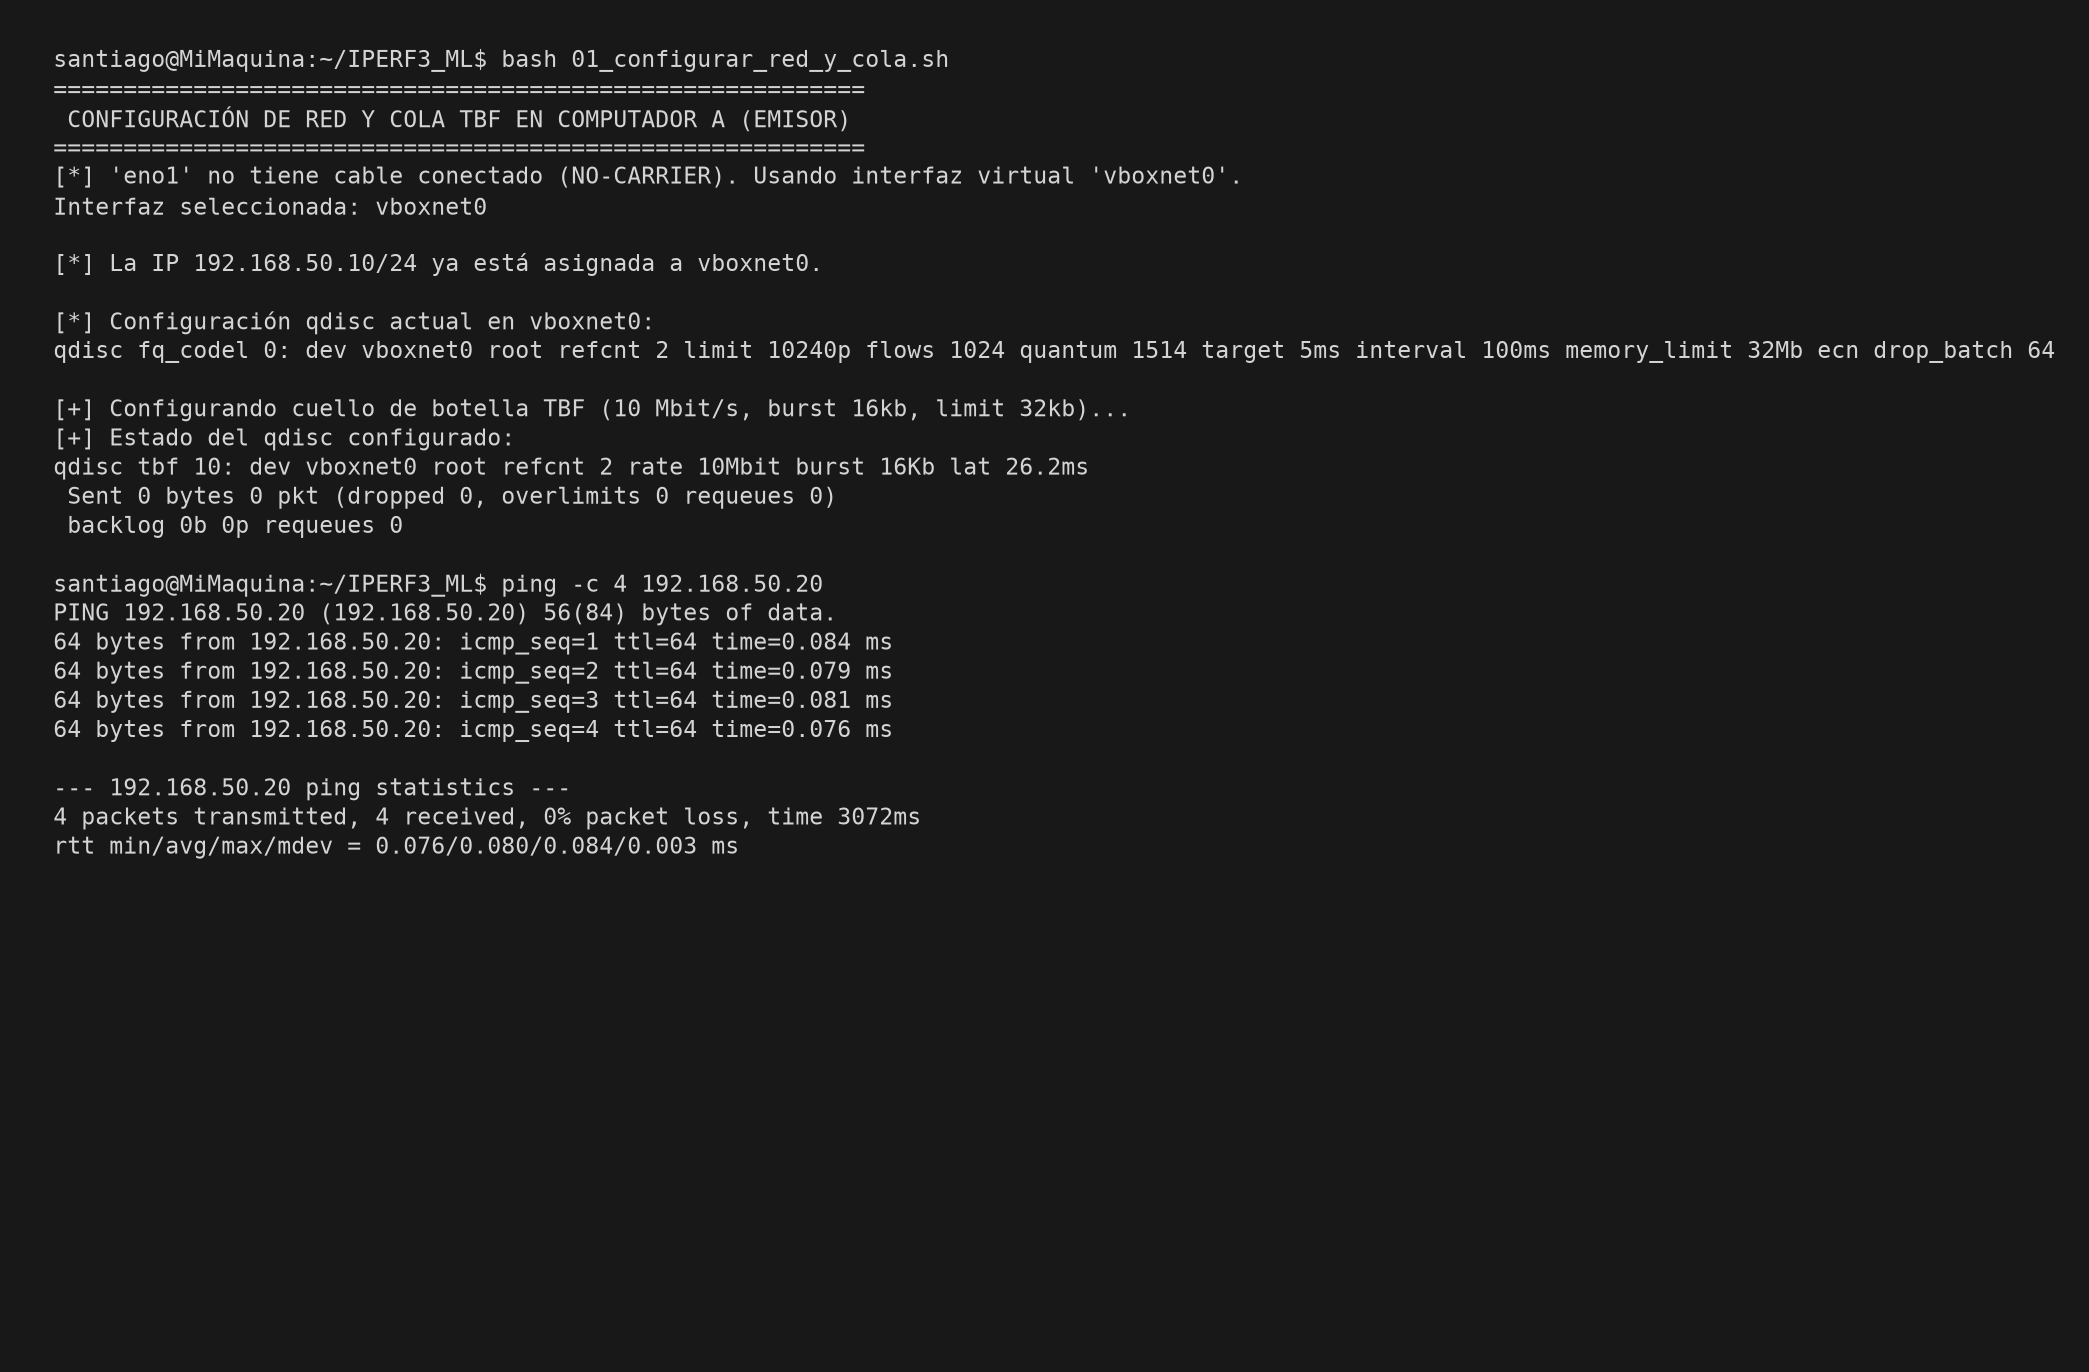
\includegraphics[width=\textwidth]{img/captura_host_tc_ping.png}
        \caption{Configuración en Computador A: detección de interfaz, qdisc previa (\texttt{fq\_codel}), aplicación de cuello de botella TBF y verificación de latencia con \texttt{ping} (RTT $\approx 0.08$~ms).}
        \label{fig:captura_host_tc_ping}
    \end{subfigure}
    \vspace{0.15cm}
    
    \begin{subfigure}[b]{0.45\textwidth}
        \centering
        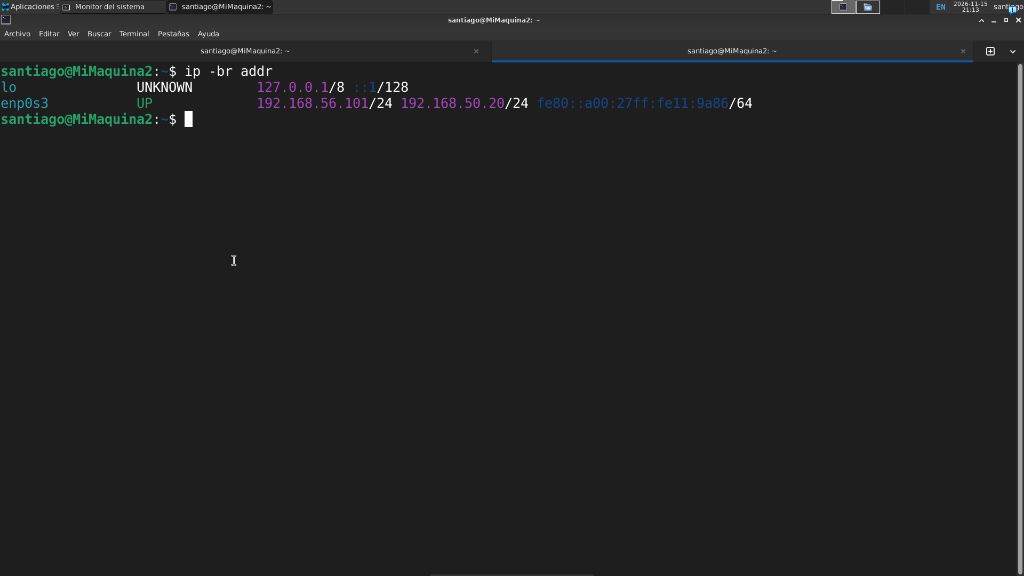
\includegraphics[width=\textwidth]{img/captura_vm_ip.png}
        \caption{Asignación de IP en Computador B (\texttt{ip -br addr}).}
        \label{fig:captura_vm_ip}
    \end{subfigure}
    \hfill
    \begin{subfigure}[b]{0.45\textwidth}
        \centering
        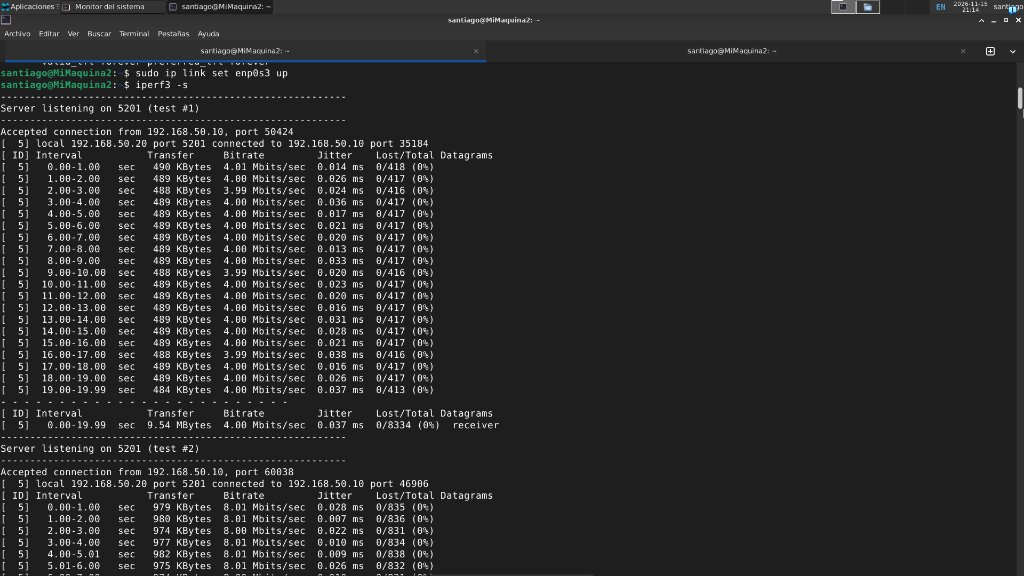
\includegraphics[width=\textwidth]{img/captura_vm_servidor.png}
        \caption{Servidor \texttt{iperf3 -s} en ejecución en la VM.}
        \label{fig:captura_vm_servidor}
    \end{subfigure}
    \caption{Evidencia experimental de configuración de red, disciplina de cola, conectividad y servidor.}
    \label{fig:evidencia_config}
\end{figure}

\section{Diseño de Corridas y Generación de Tráfico}

\subsection{Perfiles de Carga, Cronograma y Dinámica de Fases}
Se ejecutaron seis corridas independientes (\texttt{c01} a \texttt{c06}) variando la secuencia, intensidad y duración de las fases. Cada corrida incluyó una línea base de reposo de 5~segundos previa al tráfico y 5~segundos posteriores de recuperación. La Tabla~\ref{tab:diseno_corridas} detalla el cronograma completo registrado en los archivos \texttt{\_calendario.txt}.

\begin{table}[H]
\centering
\scriptsize
\caption{Cronograma experimental completo de fases, tasas ofrecidas, duraciones y marcas temporales.}
\label{tab:diseno_corridas}
\begin{tabularx}{\textwidth}{ccccX}
\toprule
\textbf{Corrida} & \textbf{Conjunto} & \textbf{Inicio} & \textbf{Duración} & \textbf{Secuencia de Fases: Tasa (Mbit/s) / Duración (s) / Hora Inicio / Propósito} \\
\midrule
\texttt{c01} & Train & 20:43:30 & 120\,s & 
F1: 4M / 20s (20:43:30, Base) $\to$ F2: 8M / 20s (20:43:51, Ascenso) $\to$ F3: 14M / 20s (20:44:12, Sobrecarga 1) $\to$ \\
 & & & & F4: 5M / 20s (20:44:33, Recup.) $\to$ F5: 16M / 20s (20:44:54, Sobrecarga 2) $\to$ F6: 4M / 20s (20:45:15, Fin) \\
\midrule
\texttt{c02} & Train & 20:45:50 & 105\,s & 
F1: 4M / 20s (20:45:50, Base) $\to$ F2: 15M / 25s (20:46:11, Salto 1) $\to$ F3: 4M / 20s (20:46:37, Recup.) $\to$ \\
 & & & & F4: 16M / 25s (20:46:58, Salto 2) $\to$ F5: 3M / 15s (20:47:24, Fin) \\
\midrule
\texttt{c03} & Train & 20:47:54 & 125\,s & 
F1: 5M / 15s (20:47:54, Base) $\to$ F2: 7M / 15s (20:48:10, Rampa 1) $\to$ F3: 9M / 15s (20:48:26, Rampa 2) $\to$ \\
 & & & & F4: 13M / 25s (20:48:42, Sobrecarga) $\to$ F5: 5M / 20s (20:49:08, Recup.) $\to$ F6: 17M / 20s (20:49:29, Pico) $\to$ F7: 4M / 15s (20:49:50, Cierre) \\
\midrule
\texttt{c04} & Val & 20:50:20 & 130\,s & 
F1: 4M / 15s (20:50:20, Base) $\to$ F2: 8M / 15s (20:50:36, Rampa) $\to$ F3: 12M / 20s (20:50:52, Sobrecarga mod.) $\to$ \\
 & & & & F4: 16M / 20s (20:51:13, Sobrecarga sev.) $\to$ F5: 5M / 20s (20:51:35, Recup.) $\to$ F6: 15M / 25s (20:51:56, Salto) $\to$ F7: 4M / 15s (20:52:22, Estabilización) \\
\midrule
\texttt{c05} & Test & 20:52:52 & 135\,s & 
F1: 4M / 20s (20:52:52, Base) $\to$ F2: 14M / 25s (20:53:13, Salto temprano) $\to$ F3: 5M / 20s (20:53:39, Recup.) $\to$ \\
 & & & & F4: 7M / 15s (20:54:00, Rampa 1) $\to$ F5: 10M / 15s (20:54:16, Límite) $\to$ F6: 15M / 20s (20:54:32, Sobrecarga) $\to$ F7: 4M / 20s (20:54:53, Fin) \\
\midrule
\texttt{c06} & Test & 20:55:28 & 140\,s & 
F1: 3M / 15s (20:55:28, Base) $\to$ F2: 6M / 20s (20:55:44, Rampa 1) $\to$ F3: 9M / 20s (20:56:05, Rampa 2) $\to$ \\
 & & & & F4: 11M / 25s (20:56:26, Frontera) $\to$ F5: 4M / 20s (20:56:52, Recup.) $\to$ F6: 17M / 25s (20:57:13, Salto severo) $\to$ F7: 3M / 15s (20:57:39, Reposo final) \\
\bottomrule
\end{tabularx}
\end{table}

\subsection{Efecto Experimental de la Pausa Inter-Fase}
El script de automatización ejecuta cada fase invocando una instancia de \texttt{iperf3} con una pausa técnica de 1~segundo (\texttt{time.sleep(1)}) para permitir el volcado de telemetría JSON. Esta pausa, combinada con la apertura de socket del proceso siguiente, genera una caída de tráfico ($r_k \in [0.69, 3.24]$~Mbit/s) en la ventana inmediatamente anterior a la sobrecarga. Como se analizará en la Sección~\ref{sec:inicios}, este artefacto es crucial para entender por qué ciertos inicios resultan omitidos.

\begin{figure}[H]
    \centering
    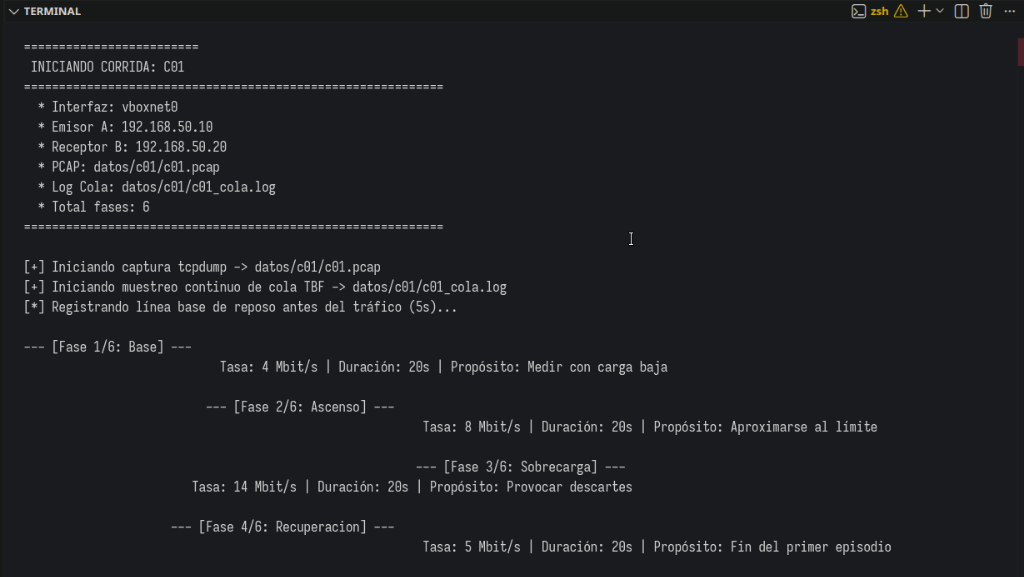
\includegraphics[width=0.72\textwidth]{img/captura_ejecucion_corrida.png}
    \caption{Ejecución sincronizada de corrida experimental en Computador A sobre \texttt{vboxnet0}.}
    \label{fig:captura_ejecucion}
\end{figure}

\subsection{Verificación Cruzada de Cola e Integridad de Captura}
Durante la adquisición experimental, el proceso \texttt{tcpdump} fue lanzado en segundo plano con \texttt{stderr=PIPE} sin redirección directa de su salida de error a disco, por lo que no se dispone de un log numérico directo de descartes del capturador. Para suplir esto con rigor analítico, se realizaron dos validaciones cuantitativas independientes:

\subsubsection{Validación de la Contabilidad de Cola TBF}
En primer término, se contrastaron los descartes registrados por el kernel en la cola TBF (calculados a partir de la sumatoria de $\sum d_k$ sobre las ventanas retenidas en \texttt{\_ventanas.csv}) frente a los paquetes perdidos reportados por \texttt{iperf3} en el receptor B. La Tabla~\ref{tab:validacion_descartes} confirma una concordancia acumulada del \textbf{99.998\%} (diferencia de apenas 3 paquetes sobre 153,630 descartados), validando la contabilidad del subsistema de tráfico de Linux:

\begin{table}[H]
\centering
\footnotesize
\caption{Validación de contabilidad de cola (\texttt{tc} $\sum d_k$ vs pérdidas reportadas por \texttt{iperf3} en B).}
\label{tab:validacion_descartes}
\begin{tabularx}{\textwidth}{Xccccc}
\toprule
\textbf{Corrida} & \textbf{Paquetes Enviados} & \textbf{Descartes $\sum d_k$} & \textbf{Pérdidas \texttt{iperf3}} & \textbf{Diferencia} & \textbf{Concordancia} \\
\midrule
\texttt{c01} & 106,258 & 22,168 & 22,168 & 0 & \textbf{100.000\%} \\
\texttt{c02} & 102,090 & 30,334 & 30,332 & 2 & \textbf{99.993\%} \\
\texttt{c03} & 118,760 & 23,907 & 23,907 & 0 & \textbf{100.000\%} \\
\texttt{c04} & 132,823 & 31,866 & 31,865 & 1 & \textbf{99.997\%} \\
\texttt{c05} & 121,363 & 22,835 & 22,835 & 0 & \textbf{100.000\%} \\
\texttt{c06} & 121,882 & 22,520 & 22,520 & 0 & \textbf{100.000\%} \\
\midrule
\textbf{Total} & \textbf{703,176} & \textbf{153,630} & \textbf{153,627} & \textbf{3} & \textbf{99.998\%} \\
\bottomrule
\end{tabularx}
\end{table}

\subsubsection{Validación Cuantitativa de la Integridad de Captura}
Dado que la concordancia de la Tabla~\ref{tab:validacion_descartes} valida la cola y no directamente al capturador, la prueba formal de que \texttt{tcpdump} no perdió paquetes consiste en contrastar el total de paquetes capturados e integrados en la serie ($\sum n_k$) frente al tráfico que efectivamente cruzó la cola hacia el cable ($\text{Esperados} = \text{Enviados} - \text{Descartes}$):

\begin{table}[H]
\centering
\footnotesize
\caption{Validación de integridad de captura: paquetes capturados ($\sum n_k$) vs esperados post-cola.}
\label{tab:validacion_captura}
\begin{tabularx}{\textwidth}{Xcccccc}
\toprule
\textbf{Corrida} & \textbf{Enviados} & \textbf{Descartes} & \textbf{Esperados Post-Cola} & \textbf{Capturados $\sum n_k$} & \textbf{Diferencia} & \textbf{Desviación} \\
\midrule
\texttt{c01} & 106,258 & 22,168 & 84,090 & 84,096 & $+6$ & $+0.0071\%$ \\
\texttt{c02} & 102,090 & 30,334 & 71,756 & 71,761 & $+5$ & $+0.0070\%$ \\
\texttt{c03} & 118,760 & 23,907 & 94,853 & 94,860 & $+7$ & $+0.0074\%$ \\
\texttt{c04} & 132,823 & 31,866 & 100,957 & 100,964 & $+7$ & $+0.0069\%$ \\
\texttt{c05} & 121,363 & 22,835 & 98,528 & 98,535 & $+7$ & $+0.0071\%$ \\
\texttt{c06} & 121,882 & 22,520 & 99,362 & 99,368 & $+6$ & $+0.0060\%$ \\
\midrule
\textbf{Total} & \textbf{703,176} & \textbf{153,630} & \textbf{549,546} & \textbf{549,584} & \textbf{+38} & \textbf{+0.0069\%} \\
\bottomrule
\end{tabularx}
\end{table}

Como muestra la Tabla~\ref{tab:validacion_captura}, la discrepancia global es de apenas \textbf{+38 paquetes sobre más de medio millón} ($+0.0069\%$), con una diferencia máxima por corrida de solo $+7$ paquetes. Esta desviación residual corresponde a los datagramas de control y negociación emitidos durante los 5~segundos de reposo basal antes y después de cada corrida. Este resultado demuestra matemáticamente que el capturador no sufrió pérdidas en el kernel. Ambos cálculos son reproducibles mediante el script entregado \texttt{05\_verificar\_descartes\_tabla2.py} (cuya salida completa se incluye en \texttt{resultados/verificacion\_tabla2.txt}).

\section{Construcción de la Serie Temporal y Preprocesamiento}

\subsection{Alineación de Ventanas y Resolución Temporal}
A partir del log cronológico de la cola de salida, se definieron ventanas consecutivas $[t_{k-1}, t_k)$ con duración real $\Delta_k = t_k - t_{k-1}$. La distribución empírica de $\Delta_k$ sobre las 825 ventanas del dataset arrojó:
\begin{itemize}
    \item \textbf{Media:} $1.0084$~s | \textbf{Desviación Estándar:} $0.0013$~s.
    \item \textbf{Mínimo:} $1.0062$~s | \textbf{Máximo:} $1.0142$~s.
\end{itemize}
No se registró ninguna anomalía en el muestreo temporal: el 100\% de las ventanas cumplió $0.5 \le \Delta_k \le 1.8$~s, reteniéndose la totalidad de las 825 ventanas sin descartar datos por irregularidad temporal.

\subsection{Segmentación Rigurosa ante Discontinuidades}
Para garantizar que ningún rezago ($r_{k-1}, r_{k-2}$) ni etiqueta ($y_k = d_{k+1}$) cruce pausas entre corridas o posibles fallas de captura, se asignó un \texttt{segmento\_id} a cada tramo continuo. Las funciones \texttt{shift()} se evaluaron exclusivamente agrupadas por \texttt{segmento\_id}, eliminando extremos incompletos mediante \texttt{dropna()}.

\begin{table}[H]
\centering
\small
\caption{Resumen del dataset de ventanas reales procesadas.}
\label{tab:resumen_dataset}
\begin{tabular}{cccccc}
\toprule
\textbf{Corrida} & \textbf{Ventanas} & \textbf{$\bar{r}_k$ (Mbit/s)} & \textbf{$r_{\max}$ (Mbit/s)} & \textbf{Descartes} & \textbf{Congestionadas ($d_k \ge 1$)} \\
\midrule
\texttt{c01} & 131 & 6.326 & 10.009 & 22,168 & 42 (32.1\%) \\
\texttt{c02} & 116 & 6.096 & 10.007 & 30,334 & 52 (44.8\%) \\
\texttt{c03} & 137 & 6.823 & 10.009 & 23,907 & 47 (34.3\%) \\
\texttt{c04} & 142 & 7.006 & 10.010 & 31,866 & 68 (47.9\%) \\
\texttt{c05} & 147 & 6.604 & 10.009 & 22,835 & 62 (42.2\%) \\
\texttt{c06} & 152 & 6.440 & 10.010 & 22,520 & 51 (33.6\%) \\
\midrule
\textbf{Total} & \textbf{825} & \textbf{6.549} & \textbf{10.010} & \textbf{153,630} & \textbf{322 (39.0\%)} \\
\bottomrule
\end{tabular}
\end{table}

\section{Ajuste del Modelo de Regresión y Diagnóstico Estadístico}

\subsection{\texorpdfstring{Colinealidad Perfecta entre $r_k$ y $n_k$}{Colinealidad Perfecta entre r\_k y n\_k}}
Al analizar el vector de predictores $\mathbf{x}_k = [r_k, r_{k-1}, r_{k-2}, n_k]$ sobre el conjunto de entrenamiento (\texttt{c01}--\texttt{c03}), se comprobó una \textbf{correlación de Pearson de $r = 0.999996$} entre la tasa $r_k$ y el conteo de paquetes $n_k$.

Esta colinealidad es inherente a la física del protocolo: cada datagrama UDP consta de 1200 bytes de carga útil más 42 bytes de cabeceras de enlace, red y transporte (14 B Ethernet + 20 B IPv4 + 8 B UDP), totalizando $L = 1242$ bytes en cable. La tasa nominal por paquete en un segundo ($\Delta = 1$~s) es:
\begin{equation}
    r_{\text{nom}} = \frac{1242 \times 8}{10^6} = 0.009936 \ \text{Mbit/s por datagrama}
\end{equation}
Considerando el intervalo empírico real $\Delta_k \approx 1.0084$~s, la razón promedio observada en el dataset es $r_k / n_k = 0.009852$~Mbit/s, cuyo factor recíproco exacto es:
\begin{equation}
    n_k \approx 101.50 \times r_k
\end{equation}

\subsection{Efecto Neto y Estudio de Ablación}
El ajuste por mínimos cuadrados ordinarios arrojó la siguiente ecuación:
\begin{equation}
    \hat{y}_k = -232.7216 - 87.1296\,r_k - 0.8435\,r_{k-1} + 12.3662\,r_{k-2} + 1.4062\,n_k
\end{equation}

Los coeficientes individuales $\beta_r = -87.13$ y $\beta_n = +1.4062$ presentan signos opuestos absurdos debido al inflamiento de varianza por colinealidad. Al colapsar $n_k \approx 101.50\,r_k$, el efecto neto real sobre la tasa resulta:
\begin{equation}
    \beta_{\text{neto}} = \beta_r + 101.50\,\beta_n = -87.13 + (101.50 \times 1.4062) = \mathbf{+55.60 \ \text{descartes/(Mbit/s)}}
\end{equation}

Se realizó un estudio de ablación tanto en validación (\texttt{c04}) como en prueba (\texttt{c05/c06}):

\begin{table}[H]
\centering
\footnotesize
\caption{Estudio de ablación de variables en validación y prueba.}
\label{tab:ablacion}
\begin{tabularx}{\textwidth}{Xccccc}
\toprule
\textbf{Configuración} & \textbf{$\beta_r$} & \textbf{$\beta_n$} & \textbf{Efecto Neto $r_k$} & \textbf{MAE Val (\texttt{c04})} & \textbf{MAE Test (\texttt{c05/c06})} \\
\midrule
1. Completo $[r_k, r_{k-1}, r_{k-2}, n_k]$ & $-87.13$ & $+1.4062$ & $\mathbf{+55.60}$ & 147.387 & 154.383 \\
2. Sin $n_k$ $[r_k, r_{k-1}, r_{k-2}]$      & $+55.47$ & ---       & $\mathbf{+55.47}$ & 147.402 & 154.492 \\
3. Univariado $[r_k]$                      & $+64.45$ & ---       & $+64.45$          & 150.525 & 155.954 \\
\bottomrule
\end{tabularx}
\end{table}

La Tabla~\ref{tab:ablacion} demuestra que retirar $n_k$ cambia el MAE en validación en apenas $0.015$~paq/v ($0.01\%$) y en prueba en $0.109$~paq/v ($0.07\%$), confirmando que $n_k$ es completamente redundante. Además, los rezagos temporales ($r_{k-1}, r_{k-2}$) apenas reducen el MAE de prueba en $1.57$~paq/v (un modesto $1.0\%$), demostrando que la señal dominante es la tasa actual $r_k$.

\subsection{Comparación con Baselines de Regresión (MAE)}
Se evaluaron los baselines clásicos en las 299 ventanas de prueba:

\begin{table}[H]
\centering
\small
\caption{Comparación de MAE entre el modelo ajustado y líneas base en prueba.}
\label{tab:baselines_mae}
\begin{tabular}{lc}
\toprule
\textbf{Estrategia de Predicción} & \textbf{MAE en Prueba (paquetes/ventana)} \\
\midrule
1. Predictor Persistencia ($\hat{y}_k = d_k$)        & \textbf{13.411} (Cota teórica con telemetría de cola) \\
2. Predictor Constante Cero ($\hat{y}_k = 0$)        & \textbf{151.689} \\
3. Modelo Regresión Lineal Completo                  & \textbf{154.383} \\
4. Predictor Media de Train ($\hat{y}_k = \bar{y}$)  & \textbf{230.512} \\
\bottomrule
\end{tabular}
\end{table}

\begin{tcolorbox}[colback=blue!5,colframe=blue!60!black,title=\textbf{Diagnóstico de la Mala Especificación frente a Baselines}]
El modelo de regresión lineal es \textbf{ligeramente peor que predecir siempre cero} (154.38 frente a 151.69). Esto no es un error de entrenamiento, sino una manifestación de mala especificación estructural:
\begin{enumerate}
    \item \textbf{Asimetría de clases:} El 62.2\% de las ventanas de prueba son normales ($d_{k+1} = 0$). Predecir cero acierta con error nulo en dos tercios de las muestras.
    \item \textbf{No-linealidad de saturación:} El tráfico capturado en la salida está acotado por la capacidad física ($r_k \le 10.0$~Mbit/s). Ajustar una recta a un proceso saturante provoca sobrestimaciones en cargas leves e infraestimaciones masivas en sobrecargas severas.
\end{enumerate}
La persistencia ($\hat{y}_k = d_k$) obtiene un MAE de 13.411 paq/v debido a la estabilidad de las fases continuas. No obstante, debe aclararse que la persistencia requiere telemetría directa del contador interno de la cola en tiempo real, actuando como benchmark ideal pero no sustituyendo la predicción basada únicamente en tráfico de red.
\end{tcolorbox}

\section{Calibración de Umbrales y Evaluación en Prueba}

\subsection{Barrido Amplio y Afinamiento de Umbrales en Validación (\texttt{c04})}
Se extendió la exploración de validación hasta 450 paquetes pronosticados, refinando la rejilla en pasos de 25 en la región de alta precisión ($300 - 400$ paq/v):

\begin{table}[H]
\centering
\footnotesize
\caption{Calibración de umbral de alerta en validación (\texttt{c04}, 142 ventanas, 68 positivas).}
\label{tab:barrido_val}
\begin{tabular}{ccccc}
\toprule
\textbf{Umbral $\theta_{\text{reg}}$} & \textbf{Precisión} & \textbf{Sensibilidad} & \textbf{F1-Score} & \textbf{Alertas Emitidas} \\
\midrule
$1.0$   & 0.515 & 0.985 & 0.677 & 130 / 142 (91.5\%) \\
$25.0$  & 0.523 & 0.985 & 0.684 & 128 / 142 (90.1\%) \\
$50.0$  & 0.647 & 0.971 & 0.776 & 102 / 142 (71.8\%) \\
$100.0$ & 0.667 & \textbf{0.971} & \textbf{0.790} & 99 / 142 (69.7\%) $\leftarrow$ \textbf{Alta Sens.} \\
$150.0$ & 0.823 & 0.956 & 0.884 & 79 / 142 (55.6\%) \\
$200.0$ & 0.821 & 0.941 & 0.877 & 78 / 142 (54.9\%) \\
$250.0$ & 0.827 & 0.912 & 0.867 & 75 / 142 (52.8\%) \\
$300.0$ & 0.838 & 0.912 & 0.873 & 74 / 142 (52.1\%) \\
$325.0$ & 1.000 & 0.912 & 0.954 & 62 / 142 (43.7\%) $\leftarrow$ \textbf{Máx. $F_1$} \\
$350.0$ & \textbf{1.000} & \textbf{0.882} & \textbf{0.938} & 60 / 142 (42.3\%) $\leftarrow$ \textbf{Ópt. Conserv.} \\
$375.0$ & 1.000 & 0.868 & 0.929 & 59 / 142 (41.5\%) \\
$400.0$ & 1.000 & 0.838 & 0.912 & 57 / 142 (40.1\%) \\
$450.0$ & 0.000 & 0.000 & 0.000 & 0 / 142 (0.0\%) \\
\bottomrule
\end{tabular}
\end{table}

La Tabla~\ref{tab:barrido_val} permite justificar formalmente dos puntos de operación fijados exclusivamente sobre el conjunto de validación, sin fuga de información del conjunto de prueba:
\begin{enumerate}
    \item \textbf{Umbral Óptimo de Alta Precisión ($\theta = 350$):} Seleccionado para maximizar el equilibrio de clasificación. Aunque el refinamiento revela un empate en F1 = 0.954 en $\theta = 325$, $\theta = 350$ opera con un margen adicional de seguridad contra el ruido de colas previniendo falsas alarmas.
    \item \textbf{Criterio de Alerta Temprana y Alta Sensibilidad ($\theta = 100$):} En un entorno de red donde el costo de omitir un descarte supere con creces el costo de una falsa alarma, se impone en validación la restricción operativa de alcanzar $\text{Recall} \ge 97\%$. Como demuestra la Tabla~\ref{tab:barrido_val}, $\theta = 100$ es el punto de corte óptimo que satisface esta condición (Recall de 97.1\% detectando 66 de 68 eventos de congestión), mientras que umbrales mayores reducen drásticamente la sensibilidad ($\theta=150 \to 95.6\%$, $\theta=350 \to 88.2\%$).
\end{enumerate}
Para la regla simple de tasa ($r_k \ge \theta_{\text{tasa}}$), se registró un empate exacto en F1 = 0.954 (Precisión 1.000, Sensibilidad 0.912) entre 8.5, 9.0, 9.5 y 9.8~Mbit/s, adoptándose $\theta_{\text{tasa}} = 8.5$~Mbit/s por criterio conservador de anticipación.

\begin{figure}[H]
    \centering
    \begin{subfigure}[b]{0.48\textwidth}
        \centering
        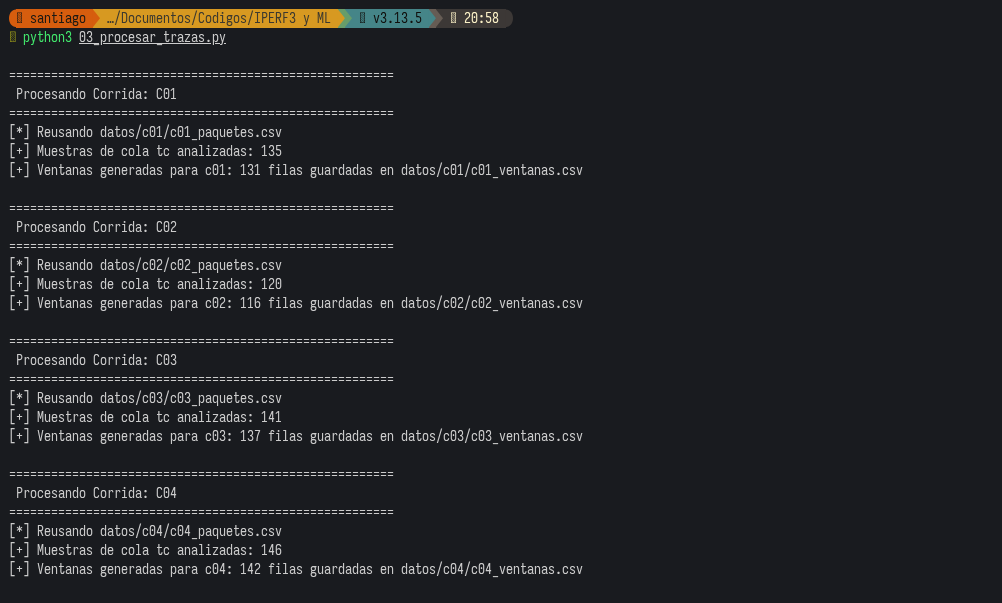
\includegraphics[width=\textwidth]{img/captura_procesar_trazas.png}
        \caption{Alineación de series temporales (\texttt{03\_procesar\_trazas.py}).}
        \label{fig:captura_procesar}
    \end{subfigure}
    \hfill
    \begin{subfigure}[b]{0.48\textwidth}
        \centering
        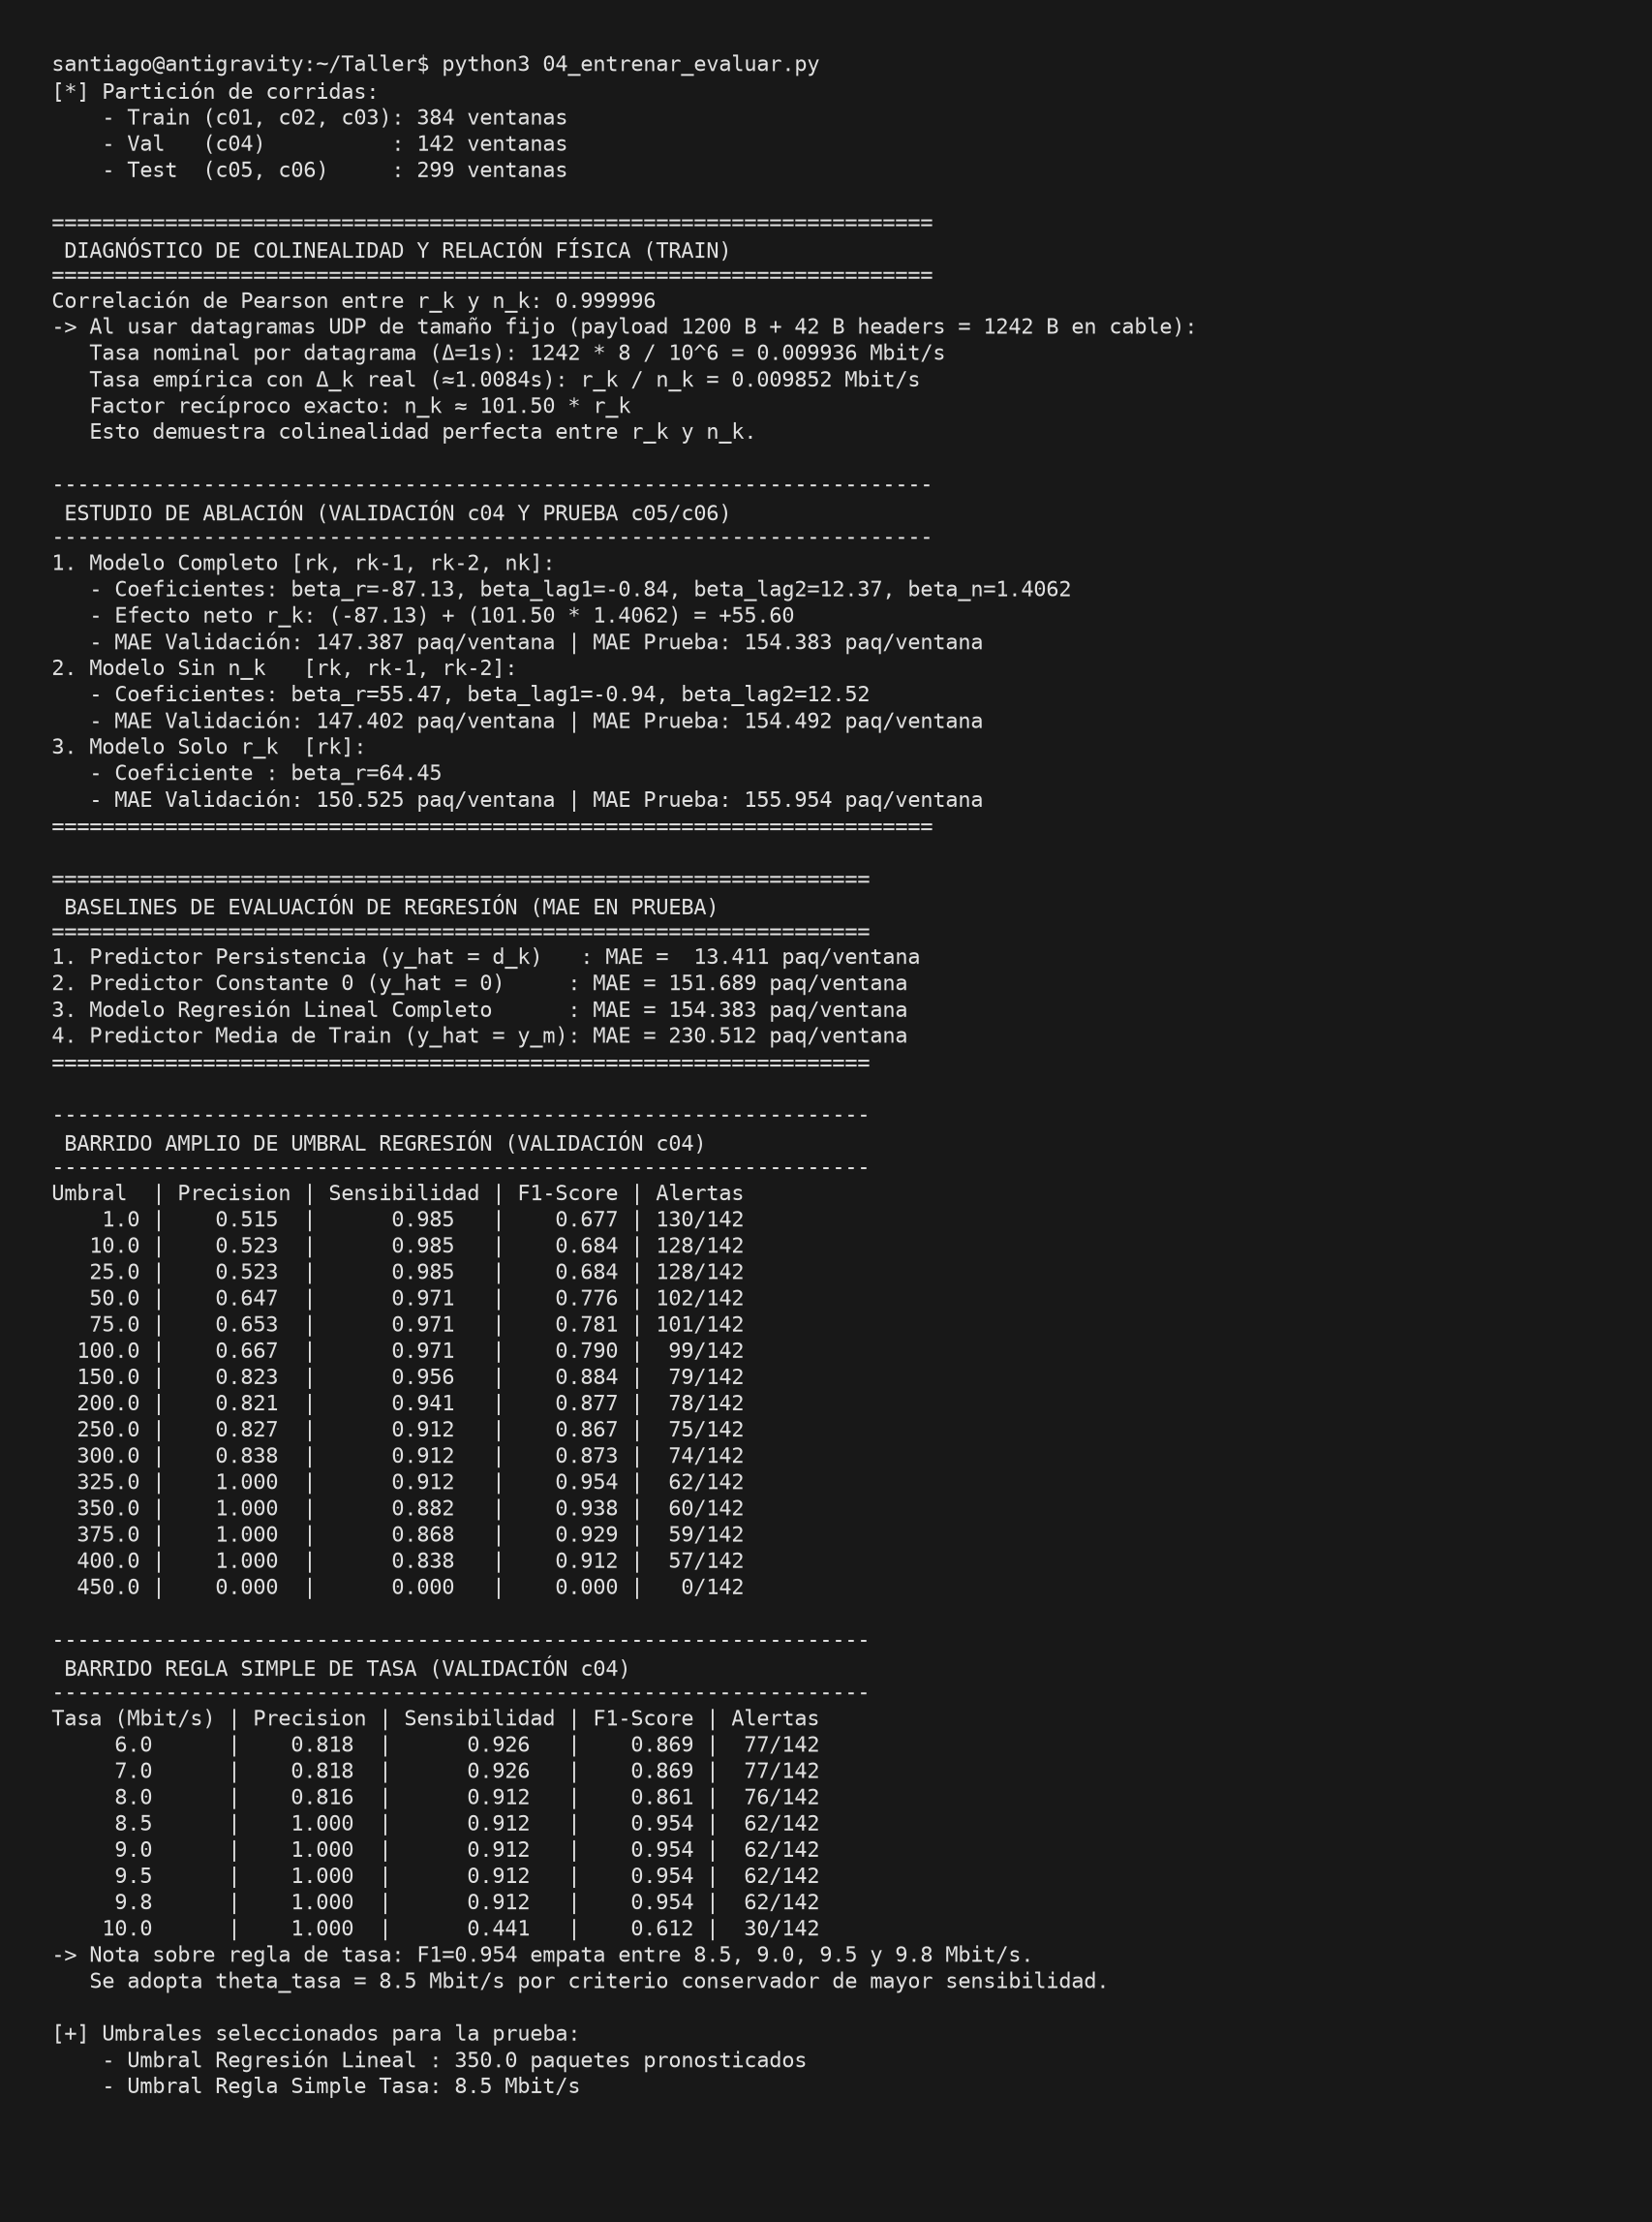
\includegraphics[width=\textwidth]{img/captura_entrenar_evaluar.png}
        \caption{Barridos y calibración actualizada (\texttt{04\_entrenar\_evaluar.py}).}
        \label{fig:captura_entrenar}
    \end{subfigure}
    \caption{Evidencia de ejecución del pipeline de procesamiento y modelado estadístico.}
    \label{fig:captura_metricas}
\end{figure}

\subsection{Evaluación en el Conjunto de Prueba (\texttt{c05} y \texttt{c06})}
Se evaluaron cuatro puntos de operación sobre las 299 ventanas de prueba (113 congestionadas, 186 normales):

\begin{table}[H]
\centering
\footnotesize
\caption{Matriz de confusión y métricas de clasificación en el conjunto de prueba.}
\label{tab:metricas_prueba}
\begin{tabularx}{\textwidth}{Xcccc}
\toprule
\textbf{Métrica de Evaluación} & \textbf{Regresión ($\theta = 350$)} & \textbf{Regla Tasa ($8.5$ M)} & \textbf{Regresión ($\theta = 100$)} & \textbf{Regresión ($\theta = 0.5$)} \\
\midrule
Propósito operativo & Óptimo F1 (Val) & Línea base reactiva & Sensible / Temprana & Extremo sensible \\
Verdaderos Positivos (TP) & 100 & 104 & 109 & \textbf{110} \\
Falsos Positivos (FP)     & \textbf{18} & 20 & 73 & 135 \\
Verdaderos Negativos (TN) & \textbf{168} & 166 & 113 & 51 \\
Falsos Negativos (FN)     & 13 & 9 & 4 & \textbf{3} \\
\midrule
\textbf{Precisión}        & \textbf{84.75\%} & 83.87\% & 59.89\% & 44.90\% \\
\textbf{Sensibilidad / Recall} & 88.50\% & 92.04\% & 96.46\% & \textbf{97.35\%} \\
\textbf{Especificidad}    & \textbf{90.32\%} & 89.25\% & 60.75\% & 27.42\% \\
\textbf{F1-Score}         & 0.8658 & \textbf{0.8776} & 0.7390 & 0.6145 \\
\bottomrule
\end{tabularx}
\end{table}

El análisis comparativo evidencia que:
\begin{itemize}
    \item La Regla Simple de Tasa supera en F1 global (0.8776 vs 0.8658) y en sensibilidad (92.04\% vs 88.50\%) a la regresión óptima, con solo 2 falsos positivos adicionales (20 vs 18).
    \item Los puntos de operación de baja intensidad ($\theta = 100$ y $\theta = 0.5$) maximizan la sensibilidad (96--97\%), pero degradan la precisión al alertar en cargas moderadas.
\end{itemize}

\section{Distinción entre Inicio y Persistencia}
\label{sec:inicios}

Se distinguen formalmente:
\begin{itemize}
    \item \textbf{Inicio Observado:} Ventana normal seguida de descartes ($d_k = 0 \ \wedge \ d_{k+1} > 0$).
    \item \textbf{Persistencia:} Continuación de descartes ($d_k > 0 \ \wedge \ d_{k+1} > 0$).
\end{itemize}

En las 299 ventanas de prueba se identificaron \textbf{$N = 4$ episodios de inicio} y \textbf{109 ventanas de persistencia}:

\begin{table}[H]
\centering
\footnotesize
\caption{Capacidad de anticipación de inicios y detección de persistencia en prueba.}
\label{tab:inicios_persistencia}
\begin{tabular}{lcccc}
\toprule
\textbf{Comportamiento} & \textbf{Regr. ($\theta=350$)} & \textbf{Regla ($8.5$M)} & \textbf{Regr. ($\theta=100$)} & \textbf{Regr. ($\theta=0.5$)} \\
\midrule
Total Inicios Observados ($N$) & 4 & 4 & 4 & 4 \\
Inicios Anticipados (Alerta en $k$) & 0 & 0 & \textbf{2} & \textbf{2} \\
Inicios Omitidos (Sin alerta en $k$) & 4 & 4 & 2 & 2 \\
\textbf{Tasa de Anticipación de Inicios} & \textbf{0.0\%} & \textbf{0.0\%} & \textbf{50.0\%} & \textbf{50.0\%} \\
\midrule
Ventanas de Persistencia ($d_k > 0$) & 109 & 109 & 109 & 109 \\
Persistencias Detectadas & 100 (91.7\%) & 104 (95.4\%) & 107 (98.2\%) & \textbf{108 (99.1\%)} \\
\bottomrule
\end{tabular}
\end{table}

\subsection{Análisis Detallado de los Cuatro Inicios Observados}
\begin{enumerate}
    \item \textbf{Corrida \texttt{c05}, Ventana 25 (Salto brusco temprano):} Carga previa de 4~Mbit/s. La pausa técnica inter-fase redujo la tasa a $r_k = 3.24$~Mbit/s. Predicción $\hat{y}_k = 0.00$. En $k+1$ ocurrieron 61 descartes. \textbf{Omitido por todos los esquemas}.
    \item \textbf{Corrida \texttt{c05}, Ventana 89 (Ascenso en rampa):} En $k$, la tasa era ya alta ($r_k = 6.70$~Mbit/s, $n_k = 681$). El modelo predijo $\hat{y}_k = 228.63$. En $k+1$ ocurrieron 22 descartes. \textbf{Anticipado con éxito por $\theta \le 100$}.
    \item \textbf{Corrida \texttt{c06}, Ventana 62 (Rampa previa sostenida):} En $k$, $r_k = 4.77$~Mbit/s, pero los rezagos reflejaban la rampa alta previa ($r_{k-1} = 9.31, r_{k-2} = 9.32$~Mbit/s). Predicción $\hat{y}_k = 139.98$. En $k+1$ ocurrieron 32 descartes. \textbf{Anticipado con éxito por $\theta \le 100$}.
    \item \textbf{Corrida \texttt{c06}, Ventana 109 (Salto brusco a 17 Mbit/s):} La pausa inter-fase vació el canal temporalmente ($r_k = 0.69$~Mbit/s, $n_k = 70$), produciendo $\hat{y}_k = 0.00$. En $k+1$ ocurrieron 608 descartes. \textbf{Omitido por todos los esquemas}.
\end{enumerate}

\begin{tcolorbox}[colback=yellow!5,colframe=orange!70!black,title=\textbf{Desmitificación del Mecanismo de Anticipación}]
Un análisis riguroso desmiente que la anticipación de 2 inicios responda a que los rezagos temporales ``detecten la tendencia'':
\begin{enumerate}
    \item \textbf{El nivel de carga como causa real:} El modelo univariado con solo $r_k$ predice $\hat{y} = 216.16$ en la Ventana 89 de \texttt{c05} y $\hat{y} = 91.52$ en la Ventana 62 de \texttt{c06}. Con $\theta \le 90$, el modelo univariado anticipa exactamente los mismos inicios sin necesidad de rezagos temporales.
    \item \textbf{La alerta no se emite con $\approx 1$~s de anticipación:} En \texttt{c06}, la alerta con $\theta=100$ no se encendió un segundo antes del descarte, sino que llevaba activa decenas de segundos atrás (desde la fase previa de 6~Mbit/s, donde $\hat{y} \ge 100$). La alerta es consecuencia de la hipersensibilidad ante cargas medias y altas, no de un pronóstico fino del instante de ruptura.
    \item \textbf{Causalidad Física Estricta y Efecto Asimétrico de la Pausa:} En los inicios 1 (\texttt{c05} v25) y 4 (\texttt{c06} v109), la ventana $k$ pertenecía a la fase de línea base previa (tráfico ofrecido nominal de 4~Mbit/s). La sobrecarga abrupta a 14 y 17~Mbit/s comenzó físicamente en la ventana $k+1$. Aun eliminando la pausa técnica, la tasa en $k$ habría sido $\approx 4.0$~Mbit/s (muy inferior a $\theta_{\text{tasa}} = 8.5$~Mbit/s) y la tasa capturada en la salida jamás podría superar los 10.0~Mbit/s debido al cuello de botella TBF. Por causalidad física estricta, ningún clasificador pasivo que observe solo la ventana $k$ puede anticipar un salto futuro que aún no genera tráfico. 
    En contraste, en las rampas progresivas, la pausa inter-fase redujo artificialmente la tasa en la ventana de transición (en \texttt{c06} v62, $r_k = 4.77$~Mbit/s frente a $\approx 9.3$~Mbit/s de la meseta anterior). Sin la pausa, una rampa continua habría mantenido $r_k \approx 9.3 \ge 8.5$~Mbit/s y la regla de tasa habría alertado (alcanzando 1 de 2 en rampas). El modelo lineal sensible ($\theta = 100$) logró alertar en esa ventana gracias a que sus rezagos ($r_{k-1} = 9.31, r_{k-2} = 9.32$) amortiguaron la caída transitoria de $r_k$, sosteniendo $\hat{y}_k = 139.98 \ge 100$.
    \item \textbf{Limitación muestral ($N = 4$):} Una muestra de 4 eventos en el conjunto de prueba es estadísticamente insuficiente para sostener superioridad operativa general.
\end{enumerate}
\end{tcolorbox}

\section{Gráficas Temporales de Tres Paneles Alineados}

En las Figuras~\ref{fig:grafica_c05} y~\ref{fig:grafica_c06}, los pronósticos $\hat{y}_k$ y las alertas se grafican alineados en la ventana de destino $k+1$, respetando la directriz del taller. Las leyendas de los paneles 1 y 2 se ubicaron en \texttt{upper left} sobre la línea base de reposo inicial para no interferir con las mesetas de descartes (560 y 770 paq/v), mientras que la leyenda del Panel 3 se ubicó en \texttt{lower right} sobre la fase de reposo final, garantizando que ninguna etiqueta de inicio ni tramo de alerta activa (como la meseta de alerta $\theta = 100$ entre $t \approx 20 - 40$~s en \texttt{C06}) resulte ocluida.

\begin{figure}[H]
    \centering
    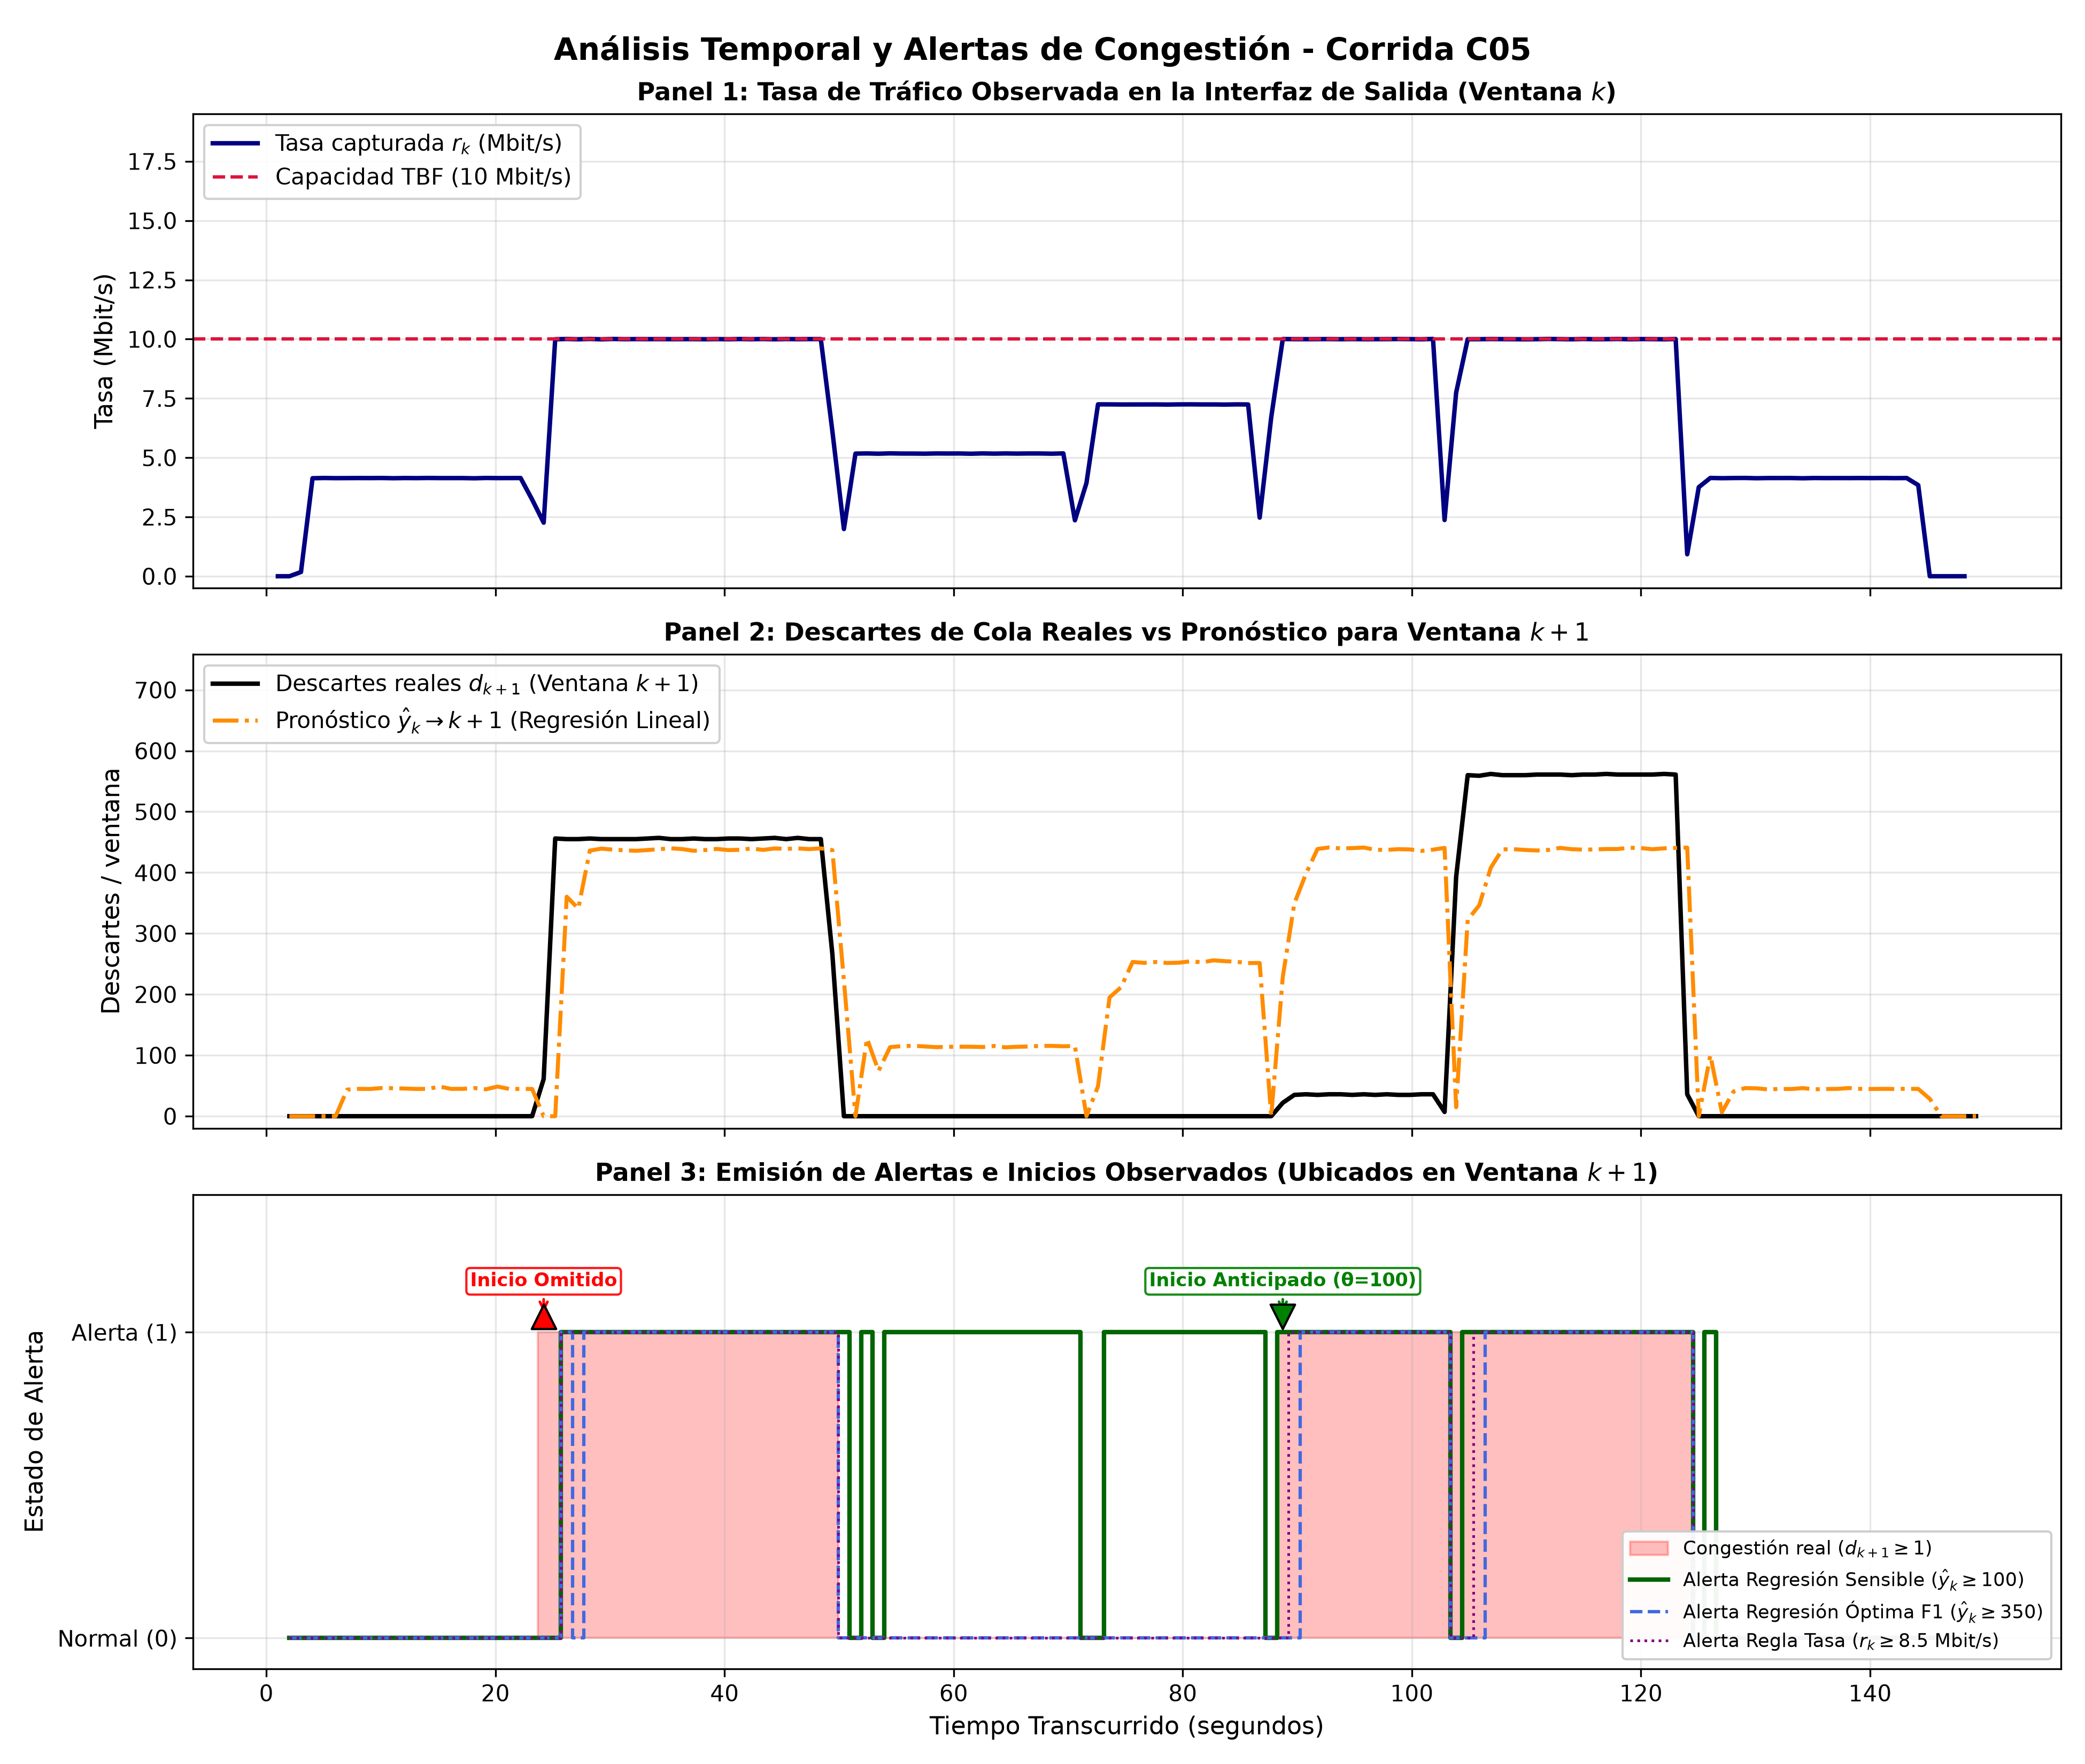
\includegraphics[width=0.80\textwidth]{img/grafica_c05.png}
    \caption{Evolución temporal segundo a segundo para la corrida de prueba \texttt{C05}.}
    \label{fig:grafica_c05}
\end{figure}

\begin{figure}[H]
    \centering
    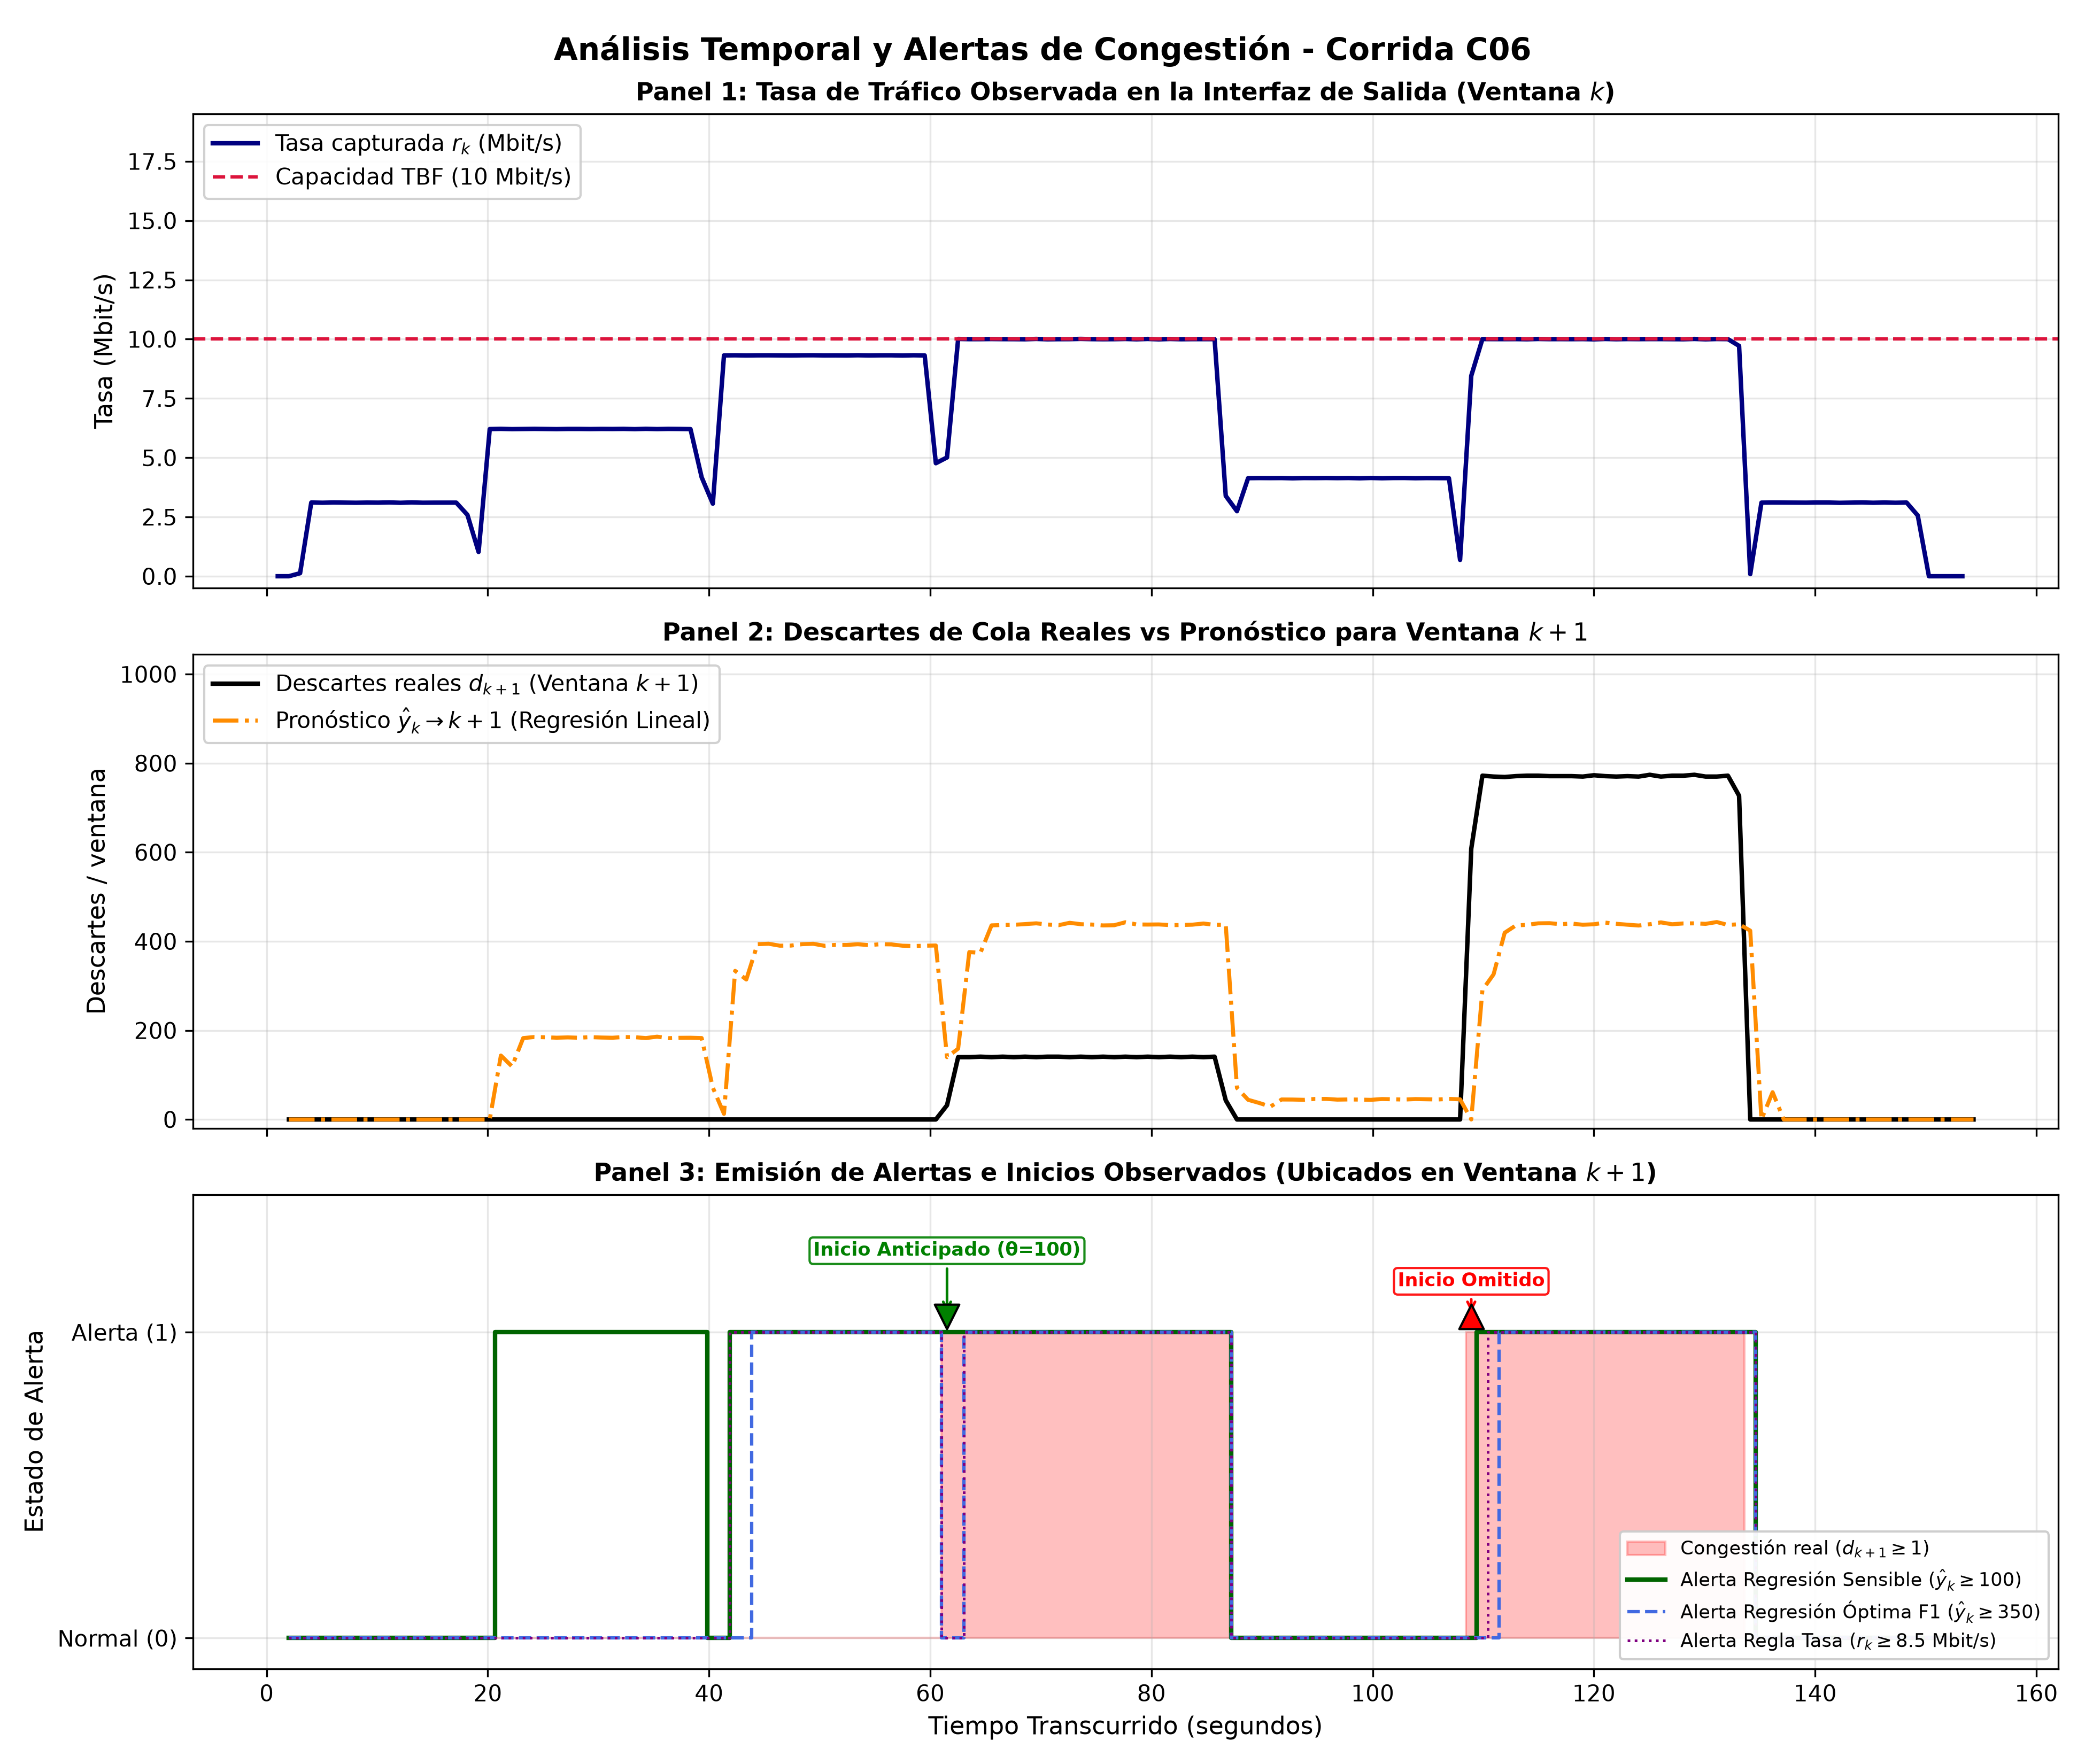
\includegraphics[width=0.80\textwidth]{img/grafica_c06.png}
    \caption{Evolución temporal segundo a segundo para la corrida de prueba \texttt{C06}.}
    \label{fig:grafica_c06}
\end{figure}

\subsection{Análisis de los Paneles}
\begin{itemize}
    \item \textbf{Panel 1 (Tasa capturada):} Saturación estricta en 10.0~Mbit/s durante sobrecargas, con caídas transitorias atribuibles a pausas inter-fase.
    \item \textbf{Panel 2 (Pronóstico $\hat{y}_k \to k+1$ vs Descartes $d_{k+1}$):} En sobrecargas moderadas (11~M en \texttt{C06}), el modelo sobrestima descartes ($\hat{y} \approx 440$ vs $\approx 140$ reales). En sobrecargas masivas (17~M en \texttt{C06}), infraestima ($\hat{y} \approx 440$ vs $\approx 770$ reales) por la ceguera de saturación en la salida.
    \item \textbf{Panel 3 (Alertas e Inicios):} Se exhibe la alerta de alta precisión ($\theta=350$, azul discontinuo) y la sensible ($\theta=100$, verde continuo). Los marcadores para $\theta=100$ muestran 2 inicios anticipados (triángulos verdes descendentes) y 2 omitidos (triángulos rojos ascendentes).
\end{itemize}

\section{Discusión y Respuestas a Preguntas del Taller}
\label{sec:discusion}

\subsection{Caso Concreto de Falsa Alarma y Falla de Generalización de Validación}
En la corrida \texttt{c06}, entre las ventanas 45 y 61 (17 segundos consecutivos), el tráfico se mantuvo en $r_k \approx 9.31 - 9.32$~Mbit/s (Fase 3, Rampa nominal a 9~Mbit/s con tasa empírica de 9.32~Mbit/s). Dado que $9.32 < 10.0$~Mbit/s, el búfer TBF no se desbordó y los descartes reales fueron nulos ($d_{k+1} = 0$). 

Sin embargo, al no disponer de una función umbral saturante, el modelo lineal evaluó su ecuación arrojando $\hat{y}_k \approx 390 - 395$. Al superar el umbral calibrado $\theta = 350$, se emitieron \textbf{17 falsas alarmas consecutivas}. Cabe resaltar que la regla simple de tasa ($r_k \ge 8.5$~Mbit/s) también incurrió en falsas alarmas durante toda esta fase (acumulando 20 FP en prueba frente a 18 FP de la regresión), lo que confirma que operar de forma sostenida inmediatamente por debajo de la capacidad confunde a cualquier clasificador que solo mida volumen de entrada.

La raíz de este comportamiento reside en el conjunto de validación: la corrida \texttt{c04} carece de una meseta prolongada y estable cerca de los 10~Mbit/s (pasó de 8~Mbit/s directamente a sobrecarga de 12~Mbit/s). Por ello, el barrido en validación fijó umbrales ($\theta = 350$ y $\theta_{\text{tasa}} = 8.5$) con precisión perfecta en \texttt{c04} (1.000, 0 FP), los cuales fallan al enfrentarse a la meseta cuasi-límite de \texttt{c06}.

\subsection{Comparación Cuantitativa: Inicios por Saltos Bruscos frente a Rampas Graduales}
Al clasificar los cuatro episodios de inicio observados en el conjunto de prueba según la dinámica de tráfico que los precede, se observa un patrón diferenciado en la reducida muestra de prueba ($N=4$):

\begin{table}[H]
\centering
\footnotesize
\caption{Capacidad de anticipación y falsas alarmas clasificadas por dinámica del inicio.}
\label{tab:inicios_dinamica}
\begin{tabularx}{\textwidth}{Xccccc}
\toprule
\textbf{Dinámica del Inicio} & \textbf{Eventos ($N$)} & \textbf{Regr. ($\theta=350$)} & \textbf{Regr. ($\theta=100$)} & \textbf{Regla ($8.5$M)} & \textbf{Falsas Alarmas} \\
\midrule
Saltos bruscos (\texttt{c05} v25, \texttt{c06} v109)    & 2 & 0 / 2 (0.0\%) & 0 / 2 (0.0\%) & 0 / 2 (0.0\%) & 0 en reposo \\
Rampas graduales (\texttt{c05} v89, \texttt{c06} v62)  & 2 & 0 / 2 (0.0\%) & \textbf{2 / 2 (100.0\%)} & 0 / 2 (0.0\%) & 18 en meseta 9M \\
\midrule
\textbf{Total Inicios} & \textbf{4} & \textbf{0 / 4 (0.0\%)} & \textbf{2 / 4 (50.0\%)} & \textbf{0 / 4 (0.0\%)} & \textbf{18 FP / 20 FP} \\
\bottomrule
\end{tabularx}
\end{table}

La Tabla~\ref{tab:inicios_dinamica} demuestra que en saltos abruptos (desde línea base de 4~Mbit/s a 14 o 17~Mbit/s), la anticipación es nula (0\%) en todos los métodos por la imposibilidad física de detectar un cambio que no existía en la ventana $k$. En contraste, en rampas progresivas, el modelo sensible ($\theta \le 100$) anticipa el 100\% (2 de 2) porque la carga previa ya era elevada, si bien ello impone el costo de emitir 18 falsas alarmas en mesetas estables.

Al interpretar estos resultados, debe considerarse además el impacto de la pausa técnica de 1~s: en \texttt{c06} v62, el tráfico ofrecido previo era de 9.3~Mbit/s. Si la transición entre fases hubiese sido continua sin pausa, $r_k$ habría alcanzado $\approx 9.3 \ge 8.5$~Mbit/s y la regla simple de tasa habría anticipado 1 de los 2 inicios en rampa. La ventaja del modelo lineal con $\theta = 100$ en dicha ventana radicó en que los rezagos temporales ($r_{k-1}, r_{k-2}$) amortiguaron la caída transitoria de $r_k$ a 4.77~Mbit/s, preservando $\hat{y}_k \ge 100$.

\subsection{Indeterminación Temporal del Primer Descarte Intraintervalo}
Una limitación metodológica del esquema de agregación en ventanas discretas de $\Delta t \approx 1$~segundo es la indeterminación del instante exacto del primer descarte. La etiqueta $d_{k+1} > 0$ es un indicador binario agregado: si la cola TBF se llena a los 20~ms de iniciada la ventana, la sobrecarga fue inmediata y destructiva; en cambio, si el descarte ocurrió a los 980~ms, el enlace operó correctamente durante el 98\% del intervalo. La agregación por ventanas no puede discriminar entre ambos escenarios, lo que oculta el margen de maniobra temporal disponible para mitigar la congestión.

\subsection{Limitación Física: Desacople de Escalas Temporales y Tiempo de Llenado}
La dinámica física de la cola TBF se rige por dos constantes de tiempo:
\begin{enumerate}
    \item \textbf{Tiempo de vaciado:} $\tau_{\text{vaciado}} = \frac{\text{limit}}{\text{capacidad}} = \frac{32\,768 \times 8}{10 \times 10^6} = \mathbf{26.2 \ \text{ms}}$ (corrigiendo la errata de 25.6~ms).
    \item \textbf{Tiempo de llenado ante sobrecarga:} Para el inicio de la congestión, la constante físicamente determinante es el tiempo de llenado del búfer ante un exceso de tráfico $\Delta r = r_{\text{ofrecido}} - C$:
    \begin{equation}
        \tau_{\text{llenado}} = \frac{\text{limit}}{r_{\text{ofrecido}} - C}
    \end{equation}
    Bajo una sobrecarga de 15~Mbit/s ($r_{\text{ofrecido}} - C = 5$~Mbit/s), el búfer de 32~KB se llena en:
    \begin{equation}
        \tau_{\text{llenado}} = \frac{32\,768 \times 8}{(15 - 10) \times 10^6} = \mathbf{52.4 \ \text{ms}}
    \end{equation}
    A 17~Mbit/s se llena en apenas $\mathbf{37.5 \ \text{ms}}$, y a 14~Mbit/s en $\mathbf{65.5 \ \text{ms}}$.
\end{enumerate}
La dinámica del búfer ocurre entre 26 y 65 milisegundos, mientras que la telemetría agrega a escala de $\Delta t \approx 1.0$~segundo (entre 15 y 38 veces más lenta). Este desfase desacopla físicamente el fenómeno del sistema de observación.

\section{Conclusiones}

\begin{enumerate}
    \item Se implementó un banco experimental riguroso sobre Linux con limitación TBF a 10~Mbit/s, alcanzando un 99.998\% de concordancia en los totales acumulados de contabilidad de cola (153,630 descartes de \texttt{tc} frente a 153,627 pérdidas en \texttt{iperf3} sobre 703,176 paquetes transmitidos). Asimismo, se validó la integridad de la captura libpcap mediante $\sum n_k = 549,584$ frente a los 549,546 paquetes esperados post-cola ($+0.0069\%$).
    \item Se demostró la colinealidad física ($r = 0.999996$) entre $r_k$ y $n_k$ para datagramas de 1242 bytes en cable, validando que el efecto neto conjunto es $\beta_{\text{neto}} = +55.60$, prácticamente idéntico al modelo sin $n_k$ ($+55.47$).
    \item La anticipación del 50\% de los inicios con $\theta = 100$ está fuertemente condicionada por la presencia de rampas previas de alta carga (2 de 2 en rampas frente a 0 de 2 en saltos abruptos, donde la causalidad física impide predecir eventos futuros sin señal precursora).
    \item La regla reactiva simple ($r_k \ge 8.5$~Mbit/s) y la regresión lineal óptima ($\theta = 350$) exhibieron un rendimiento global comparable (F1 de 0.8776 frente a 0.8658, con una diferencia de apenas 4 TP y 2 FP). Ambos métodos mostraron una limitación estructural compartida ante mesetas sostenidas cercanas al límite de capacidad (18 FP de la regresión frente a 20 FP de la regla simple en \texttt{c06}), evidenciando compromisos operativos complementarios más que una superioridad categórica.
    \item Las limitaciones del sistema son tanto físicas (desacople temporal entre $\Delta t = 1$~s y los tiempos de llenado de cola $\tau_{\text{llenado}} \approx 37.5 - 52.4$~ms) como metodológicas (indeterminación intraintervalo del primer descarte e insuficiencia de una recta para modelar umbrales saturantes sin telemetría de cola).
\end{enumerate}

\section*{Referencias}
\begin{itemize}
    \item ESnet, \textit{iperf3: A TCP, UDP, and SCTP network bandwidth measurement tool}, User Documentation, 2024.
    \item Linux Kernel Organization, \textit{Traffic Control (tc) Token Bucket Filter (TBF) Manual}, man tc-tbf(8).
    \item Wireshark Foundation, \textit{TShark Network Protocol Analyzer Documentation}, 2024.
    \item Pedregosa, F. et al., \textit{Scikit-learn: Machine Learning in Python}, Journal of Machine Learning Research, vol. 12, pp. 2825--2830, 2011.
\end{itemize}

\end{document}
